\section*{Appendix}
\begin{subappendices}

\section{Model Specification}
\label{c5:appendix:model_specification}
Let $T_i^*$ denote the true time of upgrading (increase in biopsy Gleason grade group from~1 to 2 or higher) for the ${i\mbox{-th}}$ patient included in PRIAS. Since biopsies are conducted periodically, $T_i^*$ is observed with interval censoring ${l_i < T_i^* \leq r_i}$. When upgrading is observed for the patient at his latest biopsy time $r_i$, then $l_i$ denotes the time of the second latest biopsy. Otherwise, $l_i$ denotes the time of the latest biopsy and ${r_i=\infty}$. Let $\boldsymbol{y}_{i}$ denote his observed PSA longitudinal measurements. The observed data of all $n$ patients is denoted by ${\mathcal{A}_n = \{l_i, r_i, \boldsymbol{y}_{i}; i = 1, \ldots, n\}}$.

In our joint model, the patient-specific PSA measurements over time are modeled using a linear mixed effects sub-model. It is given by (see Panel~A, Figure~\ref{c5:fig:3}):
\begin{equation}
\label{c5:eq:long_model_psa}
\begin{split}
    \log_2 \big\{y_{i}(t) + 1\big\} &= m_{i}(t) + \varepsilon_{i}(t),\\
    m_{i}(t) &= \beta_{0} + b_{0i} + \sum_{k=1}^4 (\beta_{k} + b_{ki})  B_k\Big(\frac{t-2}{2},\frac{\mathcal{K}-2}{2}\Big)\\
    & \quad + \beta_{5} \mbox{age}_i,
    \end{split}
\end{equation}
where, $m_{i}(t)$ denotes the measurement error free value of $\log_2 (\mbox{PSA} + 1)$ transformed \citep{pearson1994mixed,lin2000latent} measurements at time $t$. We model it non-linearly over time using B-splines \citep{de1978practical}. To this end, our B-spline basis function ${B_k\{(t-2)/2,(\mathcal{K}-2)/2\}}$ has three internal knots at $\mathcal{K} = \{0.5, 1.3, 3\}$ years, which are the three quartiles of the observed follow-up times. The boundary knots of the spline are at 0 and 6.3 years (95-th percentile of the observed follow-up times). We mean centered (mean 2 years) and standardized (standard deviation 2 years) the follow-up time $t$ and the knots of the B-spline $\mathcal{K}$ during parameter estimation for better convergence. The fixed effect parameters are denoted by ${\{\beta_{0},\ldots,\beta_{5}\}}$, and ${\{b_{0i}, \ldots, b_{4i}\}}$ are the patient specific random effects. The random effects follow a multivariate normal distribution with mean zero and variance-covariance matrix $\boldsymbol{W}$. The error $\varepsilon_{i}(t)$ is assumed to be t-distributed with three degrees of freedom and scale $\sigma$, and is independent of the random effects. 

To model the impact of PSA measurements on the risk of upgrading, our joint model uses a relative risk sub-model. More specifically, the hazard of upgrading denoted as $h_i(t)$, and the cumulative-risk of upgrading denoted as $R_i(t)$, at a time $t$ are (see Panel~C, Figure~\ref{c5:fig:3}):
\begin{equation}
\label{c5:eq:rel_risk_model}
\begin{split}
    h_i(t) &= h_0(t) \exp\Big(\gamma \mbox{age}_i +\alpha_{1} m_{i}(t) + \alpha_{2} \frac{\mathrm{d}m_{i}(t)}{\mathrm{d}{t}}\Big),\\
    R_i(t) &= \exp\Big\{-\int_0^{t} h_i(s)\mathrm{d}{s}\Big\},
    \end{split}
\end{equation}
where, $\gamma$ is the parameter for the effect of age. The impact of PSA on the hazard of upgrading is modeled in two ways, namely the impact of the error free underlying PSA value $m_{i}(t)$ (see Panel~A, Figure~\ref{c5:fig:3}), and the impact of the underlying PSA velocity $\mathrm{d}m_{i}(t)/\mathrm{d}{t}$ (see Panel~B, Figure~\ref{c5:fig:3}). The corresponding parameters are $\alpha_{1}$ and $\alpha_{2}$, respectively. Lastly, $h_0(t)$ is the baseline hazard at time t, and is modeled flexibly using P-splines \citep{eilers1996flexible}. More specifically:
\begin{equation*}
\log{h_0(t)} = \gamma_{h_0,0} + \sum_{q=1}^Q \gamma_{h_0,q} B_q(t, \boldsymbol{v}),
\end{equation*}
where $B_q(t, \boldsymbol{v})$ denotes the $q$-th basis function of a B-spline with knots $\boldsymbol{v} = v_1, \ldots, v_Q$ and vector of spline coefficients $\gamma_{h_0}$. To avoid choosing the number and position of knots in the spline, a relatively high number of knots (e.g., 15 to 20) are chosen and the corresponding B-spline regression coefficients $\gamma_{h_0}$ are penalized using a differences penalty \citep{eilers1996flexible}.

\section{Full Results}
\label{c5:appendix:full_results}
Characteristics of the six validation cohorts from the GAP3 database~\citep{gap3_2018} are shown in Table~\ref{c5:tab:gap3_summary_1}, Table~\ref{c5:tab:gap3_summary_2}, and Table~\ref{c5:tab:gap3_summary_3}. The cause-specific cumulative upgrading-risk in these cohorts is shown in Figure~\ref{c5:fig:app1}.

\begin{figure}
\centerline{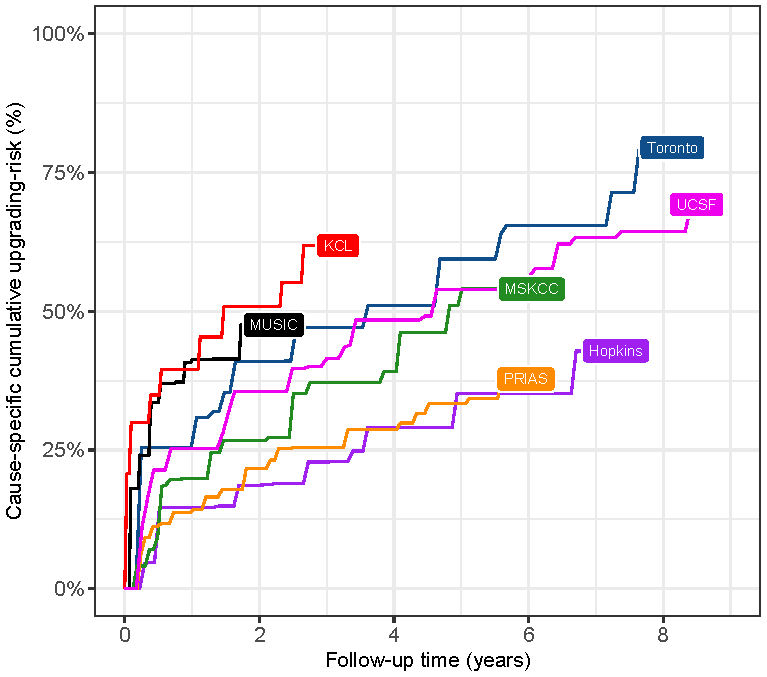
\includegraphics{contents/c5/images/c5_fig_app1.pdf}}
\caption{\textbf{Nonparametric estimate \citep{turnbull1976empirical} of the cause-specific cumulative upgrading-risk} in the world's largest AS cohort PRIAS, and largest six AS cohorts from the GAP3 database \citep{gap3_2018}. Abbreviations are \textit{Hopkins}: Johns Hopkins Active Surveillance, \textit{PRIAS}: Prostate Cancer International Active Surveillance, \textit{Toronto}: University of Toronto Active Surveillance, \textit{MSKCC}: Memorial Sloan Kettering Cancer Center Active Surveillance, \textit{KCL}: King's College London Active Surveillance, \textit{MUSIC}: Michigan Urological Surgery Improvement Collaborative AS, \textit{UCSF}: University of California San Francisco Active Surveillance.}
\label{c5:fig:app1}
\end{figure}

\begin{table}
\small
\centering
\caption{\textbf{Summary of the Hopkins and Toronto validation cohorts from the GAP3 database~\citep{gap3_2018}}. The primary event of interest is upgrading, that is, increase in Gleason grade group from group~1 to 2 or higher. \#PSA: number of PSA, \#biopsies: number of biopsies, IQR:~interquartile range, PSA:~prostate-specific antigen. Full names of cohorts are \textit{Hopkins}: Johns Hopkins Active Surveillance, \textit{Toronto}: University of Toronto Active Surveillance}
\label{c5:tab:gap3_summary_1}
\begin{tabular}{p{5cm}rr}
\hline
\textbf{Characteristic} & \textbf{Hopkins} & \textbf{Toronto}\\
\hline
Total patients & 1392 & 1046\\
Upgrading (primary event) & 260 & 359\\
\hline
Median age (years) & 62 (IQR: 66--69) & 67 (IQR: 60--72)\\
Median maximum follow-up per patient (years) &  3 (IQR: 1.3--5.8) & 4.5 (IQR: 1.9--8.4)\\
Total PSA measurements & 11126 & 13984\\
Median \#PSA per patient &  6 (IQR: 4--11) & 12 (IQR: 7--19)\\
Median PSA (ng/mL) & 4.7 (IQR: 2.9--6.7) & 6 (IQR: 3.7--9.0)\\
Total biopsies & 1926 & 909\\
Median \#biopsies per patient &  1 (IQR: 1--2) &  1 (IQR: 1--2)\\
\hline
\end{tabular}
\end{table}

\begin{table}
\small
\centering
\caption{\textbf{Summary of the MSKCC and UCSF validation cohorts from the GAP3 database~\citep{gap3_2018}}. The primary event of interest is upgrading, that is, increase in Gleason grade group from group~1 to 2 or higher. \#PSA: number of PSA, \#biopsies: number of biopsies, IQR:~interquartile range, PSA:~prostate-specific antigen. Full names of cohorts are \textit{MSKCC}: Memorial Sloan Kettering Cancer Center Active Surveillance, \textit{UCSF}: University of California San Francisco Active Surveillance.}
\label{c5:tab:gap3_summary_2}
\begin{tabular}{p{5cm}rr}
\hline
\textbf{Characteristic} & \textbf{MSKCC} & \textbf{UCSF}\\
\hline
Total patients & 894 & 1397 \\
Upgrading (primary event) & 242 & 547\\
\hline
Median age (years) & 63 (IQR: 57--68) & 63 (IQR: 57--68)\\
Median maximum follow-up per patient (years) & 5.3 (IQR: 1.8--8.3) & 3.6 (IQR: 1.5--7.2)\\
Total PSA measurements & 10704 & 16093\\
Median \#PSA per patient & 11 (IQR: 5--17) & 8 (IQR: 4--16)\\
Median PSA (ng/mL) & 4.7 (IQR: 2.8--7.1) & 5.0 (IQR: 3.4--7.2)\\
Total biopsies & 1102 & 3512\\
Median \#biopsies per patient & 1 (IQR: 1--2) & 2 (IQR: 2--3)\\
\hline
\end{tabular}
\end{table}

\begin{table}
\small
\centering
\caption{\textbf{Summary of the MUSIC and KCL validation cohorts from the GAP3 database~\citep{gap3_2018}}. The primary event of interest is upgrading, that is, increase in Gleason grade group from group~1 to 2 or higher. \#PSA: number of PSA, \#biopsies: number of biopsies, IQR:~interquartile range, PSA:~prostate-specific antigen. Full names of cohorts are \textit{KCL}: King's College London Active Surveillance, \textit{MUSIC}: Michigan Urological Surgery Improvement Collaborative AS.}
\label{c5:tab:gap3_summary_3}
\begin{tabular}{p{5cm}rr}
\hline
\textbf{Characteristic} & \textbf{MUSIC} & \textbf{KCL}\\
\hline
Total patients & 2743 & 616\\
Upgrading (primary event) & 385 & 198\\
\hline
Median age (years) & 65 (IQR: 60--71) & 63 (IQR: 58--68)\\
Median maximum follow-up per patient (years) & 1.2 (IQR: 0.6--2.2) & 2.4 (IQR: 1.3--3.8)\\
Total PSA measurements & 12087 & 2987\\
Median \#PSA per patient & 4 (IQR: 2--6) & 4 (IQR: 2--6)\\
Median PSA (ng/mL) & 5.1 (IQR: 3.4--7.1) & 6 (IQR: 4--9)\\
Total biopsies & 1032 & 484\\
Median \#biopsies per patient & 1 (IQR: 1--1) & 1 (IQR: 1--1)\\
\hline
\end{tabular}
\end{table}

For the relative risk sub-model, the parameter estimates in Table~\ref{c5:tab:PSA_survival} show that ${\log_2 (\mbox{PSA} + 1)}$ velocity and age of the patient were significantly associated with the hazard of upgrading.

\begin{table}
\small
\centering
\caption{\textbf{Parameters of the relative risk sub-model}: Estimated mean and 95\% credible interval for the parameters of the relative-risk sub-model.}
\label{c5:tab:PSA_survival}
\begin{tabular}{lrrrrr}
\hline
Variable                      & Mean   & Std. Dev & 2.5\%  & 97.5\%                 & P              \\
\hline
Age                      & 0.037    & 0.006 & 0.025  & 0.049  & \textless0.001 \\
Fitted $\log_2 (\mbox{PSA} + 1)$ value            & -0.012   & 0.076 & -0.164 & 0.135  & 0.856 \\
Fitted $\log_2 (\mbox{PSA} + 1)$ velocity             & 2.266    & 0.299 & 1.613  & 2.767  & \textless0.001   \\
\hline
\end{tabular}
\end{table}

It is important to note that since age, and ${\log_2 (\mbox{PSA} + 1)}$ value and velocity are all measured on different scales, a comparison between the corresponding parameter estimates is not easy. To this end, in Table \ref{c5:tab:PSA_survival_easy}, we present the hazard ratio of upgrading, for an increase in the aforementioned variables from their 25-th to the 75-th percentile. For example, an increase in fitted $\log_2 (\mbox{PSA} + 1)$ velocity from -0.085 to 0.308 (fitted 25-th and 75-th percentiles) corresponds to a hazard ratio of 2.433. The interpretation of the rest is similar.

\begin{table}
\small
\centering
\caption{\textbf{Hazard ratio and 95\% credible interval (CI) for upgrading}: Variables are on different scale and hence we compare an increase in the variables of relative risk sub-model from their 25-th percentile ($\mbox{P}_{25}$) to their 75-th percentile ($\mbox{P}_{75}$). Except for age, quartiles for all other variables are based on their fitted values obtained from the joint model fitted to the PRIAS dataset.}
\label{c5:tab:PSA_survival_easy}
\begin{tabular}{lrrr}
\hline
Variable                      & $\mbox{P}_{25}$   & $\mbox{P}_{75}$ & Hazard ratio [95\% CI] \\
\hline
Age & 61 & 71 & 1.455 [1.285, 1.631] \\
Fitted $\log_2 (\mbox{PSA} + 1)$ value & 2.360 & 3.078 & 0.991 [0.889, 1.102] \\
Fitted $\log_2 (\mbox{PSA} + 1)$ velocity & -0.085 & 0.308 & 2.433 [1.883, 2.962] \\
\hline
\end{tabular}
\end{table}

\begin{table}
\small
\centering
\caption{\textbf{Parameters of the relative risk sub-model in validation cohorts}. We fitted separate joint models for each of the six GAP3 validation cohorts as well. The specification of these joint models was same as that of the model for PRIAS. Two important predictors in the relative-risk sub-model, namely, the $\log_2 (\mbox{PSA} + 1)$ value and velocity have different impact on upgrading-risk across the cohorts. Table shows the mean estimate of these parameters with 95\% credible interval in brackets. Strongest average effect of $\log_2 (\mbox{PSA} + 1)$ velocity is in PRIAS cohort, whereas the weakest is in MUSIC cohort. The strongest average effect of $\log_2 (\mbox{PSA} + 1)$ value is in the Toronto cohort whereas the weakest is in PRIAS cohort. Full names of cohorts are \textit{Hopkins}: Johns Hopkins Active Surveillance, \textit{PRIAS}: Prostate Cancer International Active Surveillance, \textit{Toronto}: University of Toronto Active Surveillance, \textit{MSKCC}: Memorial Sloan Kettering Cancer Center Active Surveillance, \textit{KCL}: King's College London Active Surveillance, \textit{MUSIC}: Michigan Urological Surgery Improvement Collaborative AS, \textit{UCSF}: University of California San Francisco Active Surveillance.}
\label{c5:tab:PSA_survival_gap3}
\begin{tabular}{lrr}
\hline
Cohort & Fitted $\log_2 (\mbox{PSA} + 1)$ value & Fitted $\log_2 (\mbox{PSA} + 1)$ velocity\\
\hline
PRIAS & -0.012 [-0.164, 0.135] & 2.266 [ 1.613, 2.767]\\
Hopkins & 0.061 [-0.323, 0.329] & 1.839 [ 0.761, 4.378]\\
MSKCC & 0.336 [ 0.081, 0.583] & 1.122 [ 0.421, 1.980]\\
Toronto & 0.572 [ 0.347, 0.794] & 0.943 [ 0.464, 1.554]\\
UCSF & 0.498 [ 0.326, 0.673] & 0.812 [ 0.280, 1.383]\\
MUSIC & 0.441 [ 0.092, 0.767] & 0.029 [-0.552, 0.512]\\
KCL &  0.194 [-0.104, 0.540] & 0.840 [-0.087, 1.665]\\
\hline
\end{tabular}
\end{table}

\section{Risk Predictions for Upgrading}
\label{c5:appendix:validation_res}
Let us assume a new patient $j$, for whom we need to estimate the upgrading-risk. Let his current follow-up visit time be $v$, latest time of biopsy be $t$, observed vector PSA measurements be $\mathcal{Y}_{j}(v)$. The combined information from the observed data about the time of upgrading, is given by the following posterior predictive distribution $g(T^*_j)$ of his time $T^*_j$ of upgrading:
\begin{equation*}
\label{c5:eq:post_pred_dist}
\begin{aligned}
g(T^*_j) &= p\big\{T^*_j \mid T^*_j > t, \mathcal{Y}_{j}(v), \mathcal{A}_n\big\}\\
&= \int \int p\big(T^*_j \mid T^*_j > t, \boldsymbol{b}_j, \boldsymbol{\theta}\big) p\big\{\boldsymbol{b}_j \mid T^*_j>t, \mathcal{Y}_{j}(v), \boldsymbol{\theta}\big\}p\big(\boldsymbol{\theta} \mid \mathcal{A}_n\big) \mathrm{d} \boldsymbol{b}_j \mathrm{d} \boldsymbol{\theta}.
\end{aligned}
\end{equation*}
The distribution $g(T^*_j)$ depends not only depends on the observed data of the patient $T^*_j > t, \mathcal{Y}_{j}(v)$, but also depends on the information from the PRIAS dataset $\mathcal{A}_n$. To this the the posterior distribution of random effects $\boldsymbol{b}_j$ and posterior distribution of the vector of all parameters $\boldsymbol{\theta}$ are utilized, respectively. The distribution $g(T^*_j)$ can be estimated as detailed in \citet{rizopoulos2017dynamic}. Since, many prostate cancer patients may not obtain upgrading in the current follow-up period of PRIAS, $g(T^*_j)$ can only be estimated for a currently limited follow-up period.

The cause-specific cumulative upgrading-risk can be derived from $g(T^*_j)$ as given in~\citep{rizopoulos2017dynamic}. It is given by:
\begin{equation}
\label{c5:eq:dynamic_risk_prob}
R_j(u \mid t, v) = \mbox{Pr}\big\{T^*_j > u \mid T^*_j > t, \mathcal{Y}_{j}(v), \mathcal{A}_n\big\}, \quad u \geq t.
\end{equation}
The personalized risk profile of the patient updates as more data is gathered over follow-up visits. 

\subsection{Validation of Risk Predictions}
\label{c5:appendix:validation}
We wanted to check the usefulness of our model for not only the PRIAS patients but also for patients from other cohorts. To this end, we validated our model in the PRIAS dataset (internal validation) and the largest six cohorts from the GAP3 database~\citep{gap3_2018}. These are the University of Toronto AS (Toronto), Johns Hopkins AS (Hopkins), Memorial Sloan Kettering Cancer Center AS (MSKCC), University of California San Francisco Active Surveillance (UCSF), King's College London AS (KCL), Michigan Urological Surgery Improvement Collaborative AS (MUSIC).

\textbf{\textit{Calibration-in-the-large}}
We first assessed calibration-in-the-large~\citep{steyerberg2010assessing} of our model in the aforementioned cohorts. To this end, we used our model to predict the cause-specific cumulative upgrading-risk for each patient, given their PSA measurements and biopsy results. We then averaged the resulting profiles of cause-specific cumulative upgrading-risk. Subsequently, we compared the averaged cumulative-risk profile with a non-parametric estimate~\citep{turnbull1976empirical} of the cause-specific cumulative upgrading-risk in each of the cohorts. The results are shown in Panel~A of Figure~\ref{c5:fig:calib_before_after}. We can see that our model is miscalibrated in external cohorts, although it is fine in the Hopkins cohort. To improve our model's calibration in all cohorts, we recalibrated the baseline hazard of the joint model fitted to the PRIAS dataset, individually for each of the cohorts except the Hopkins cohort. More specifically, given the data of an external cohort $\mathcal{A}^c$, where $c$ denotes the cohort, the recalibrated parameters $\boldsymbol{\gamma}_{h_0}^c$ (Section~\ref{c5:appendix:model_specification}) of the log baseline hazard are given by:
\begin{equation}
p(\boldsymbol{\gamma}_{h_0}^c \mid \mathcal{A}^c, \boldsymbol{b^c},  \boldsymbol{\theta}) \propto \prod_{i=1}^{n^c} p(l_i^c, r_i^c \mid \boldsymbol{b^c_i}, \boldsymbol{\theta}) p(\boldsymbol{\gamma}_{h_0}^c)
\end{equation}
where $n^c$ are the number of patients in the $c$-th cohort, and $\boldsymbol{\theta}$ is the vector of all parameters of the joint model fitted to the PRIAS dataset. The interval in which upgrading is observed for the $i$-th patient is given by $l_i^c, r_i^c$, with $r_i^c = \infty$ for right-censored patients. The symbol $\boldsymbol{b^c_i}$ denotes patient-specific random effects (Section~\ref{c5:appendix:model_specification}) in the $c$-th cohort. The random effects are obtained using the joint model fitted to the PRIAS dataset before recalibration. We re-evaluated the calibration-in-the-large of our model after the recalibration of the baseline hazard individually for each cohort. The improved calibration-in-the-large is shown in Panel~B of Figure~\ref{c5:fig:calib_before_after}.

\begin{figure}
\centerline{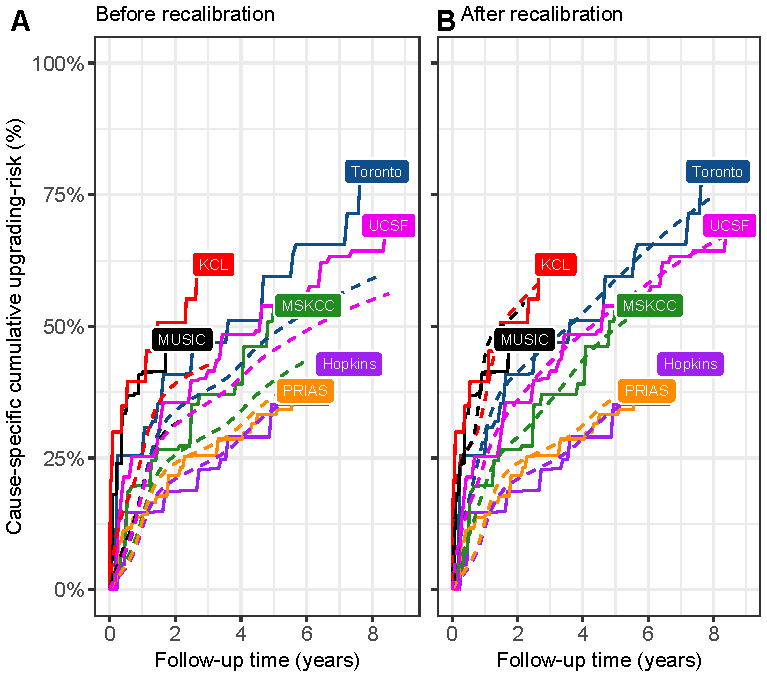
\includegraphics{contents/c5/images/c5_fig_app2.pdf}}
\caption{\textbf{Calibration-in-the-large of our model:}. In \textbf{Panel~A} we can see that our model is not well calibrated for use in KCL, MUSIC, Toronto and MSKCC. In \textbf{Panel~B} we can see that calibration of model predictions improved in KCL, MUSIC, Toronto and MSKCC cohorts after recalibrating our model. Recalibration was not necessary for Hopkins cohort. Full names of Cohorts are \textit{PRIAS}: Prostate Cancer International Active Surveillance, \textit{Toronto}: University of Toronto Active Surveillance, \textit{Hopkins}: Johns Hopkins Active Surveillance, \textit{MSKCC}: Memorial Sloan Kettering Cancer Center Active Surveillance, \textit{KCL}: King's College London Active Surveillance, \textit{MUSIC}: Michigan Urological Surgery Improvement Collaborative Active Surveillance, \textit{UCSF}: University of California San Francisco Active Surveillance.}
\label{c5:fig:calib_before_after}
\end{figure}


\textbf{\textit{Recalibrated PRIAS Model Versus Individual Joint Models For Each Cohort}}
We wanted to check if our recalibrated PRIAS model performed as good as a new joint model that could be fitted to the external cohorts. To this end, we predicted cause-specific cumulative upgrading-risk for each patient from each cohort using two sets of models, namely the recalibrated PRIAS model for each cohort, and a new joint model fitted to each cohort. The difference in predicted cause-specific cumulative upgrading-risk from these models is shown in Figure~\ref{c5:fig:calib_in_small}. We can see that the difference is smaller in those cohorts in which the effects of $\log_2 (\mbox{PSA} + 1)$ value and velocity were similar to that of PRIAS~(Table~\ref{c5:tab:PSA_survival_gap3}). For example, the Hopkins cohort had parameter estimates similar to that of PRIAS, and consequently, the difference in predicted risks for this cohort is smallest. The opposite of this phenomenon holds for the MUSIC and KCL cohorts.
 
\begin{figure}
\centerline{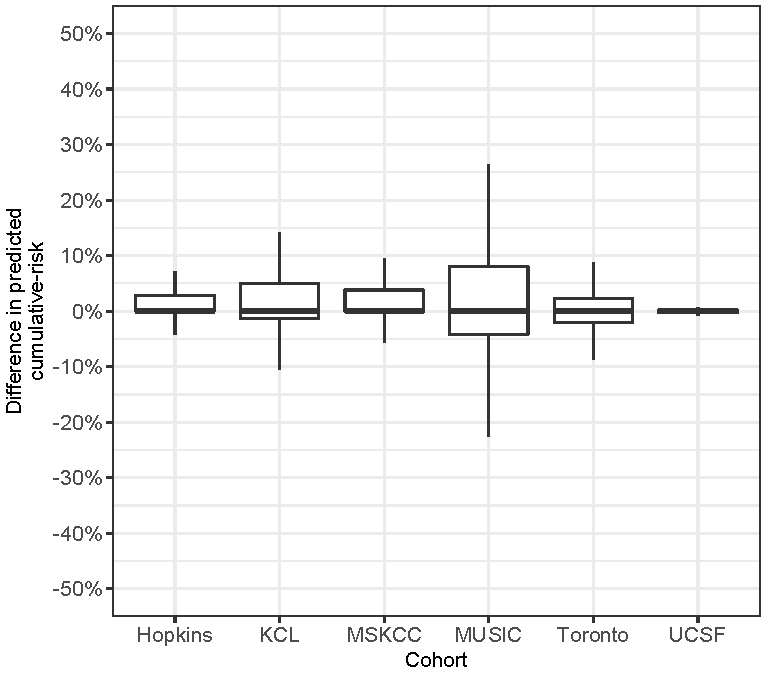
\includegraphics{contents/c5/images/c5_fig_app3.pdf}}
\caption{\textbf{Comparison of predictions from recalibrated PRIAS model with individual joint models fitted to external cohorts:} On Y-axis we show the difference between predicted cause-specific cumulative upgrading-risk for individual patients using two models, namely the recalibrated PRIAS model for each cohort, and individual joint model fitted to each cohort. The figure shows that the difference is smaller in those cohorts in which the effects of $\log_2 (\mbox{PSA} + 1)$ value and velocity were similar to that of PRIAS~(Table~\ref{c5:tab:PSA_survival_gap3}). Full names of Cohorts are \textit{PRIAS}: Prostate Cancer International Active Surveillance, \textit{Toronto}: University of Toronto Active Surveillance, \textit{Hopkins}: Johns Hopkins Active Surveillance, \textit{MSKCC}: Memorial Sloan Kettering Cancer Center Active Surveillance, \textit{KCL}: King's College London Active Surveillance, \textit{MUSIC}: Michigan Urological Surgery Improvement Collaborative Active Surveillance, \textit{UCSF}: University of California San Francisco Active Surveillance.}
\label{c5:fig:calib_in_small}
\end{figure}

\textbf{\textit{Validation of Dynamic Cumulative-Risk Predictions}}
The cumulative-risk predictions from the joint model are dynamic in nature. That is, they update as more data becomes available over time. Consequently, the discrimination and prediction error of the joint model also depend on the available data. We assessed these two measures dynamically in the PRIAS cohort (interval validation) and in the largest six external cohorts that are part of the GAP3 database. For discrimination, we utilized the time-varying area under the receiver operating characteristic curve or time-varying AUC~\citep{rizopoulos2017dynamic}. For time-varying prediction error, we assessed the mean absolute prediction error or MAPE~\citep{rizopoulos2017dynamic}. The AUC indicates how well the model discriminates between patients who experience upgrading, and those do not. The MAPE indicates how accurately the model predicts upgrading. Both AUC and MAPE are restricted to $[0,1]$. However, it is preferred that AUC $>$ 0.5 because an AUC $\leq$ 0.5 indicates that the model performs worse than random discrimination. Ideally, MAPE should be 0.

We calculate AUC and MAPE in a time-dependent manner. More specifically, given the time of latest biopsy $t$, and history of PSA measurements up to time $v$, we calculate AUC and MAPE for a medically relevant time frame $(t, v]$, within which the occurrence of upgrading is of interest. In the case of prostate cancer, at any point in time $v$, it is of interest to identify patients who may have experienced upgrading in the last one year $(v-1, v]$. That is, we set $t=v-1$. We then calculate AUC and MAPE at a gap of every six months (follow-up schedule of PRIAS). That is, $v \epsilon \{1, 1.5, \ldots \}$ years. To obtain reliable estimates of AUC and MAPE, in each cohort, we restrict $v$ to a maximum time point $v_{\mbox{max}}$, such that there are at least ten patients who experience upgrading after $v_{\mbox{max}}$. This maximum time point $v_{\mbox{max}}$ differs between cohorts, and is given in Table~\ref{c5:tab:max_pred_time}.

\begin{table}
\small
\centering
\caption{\textbf{Maximum follow-up period up to which we can reliably predict upgrading-risk and create personalized schedules}. In each cohort, this time point is chosen such that there are at least 10 patients who experience upgrading after this time point. Full names of Cohorts are \textit{PRIAS}: Prostate Cancer International Active Surveillance, \textit{Toronto}: University of Toronto Active Surveillance, \textit{Hopkins}: Johns Hopkins Active Surveillance, \textit{MSKCC}: Memorial Sloan Kettering Cancer Center Active Surveillance, \textit{KCL}: King's College London Active Surveillance, \textit{MUSIC}: Michigan Urological Surgery Improvement Collaborative Active Surveillance, \textit{UCSF}: University of California San Francisco Active Surveillance.}
\label{c5:tab:max_pred_time}
\begin{tabular}{l|r}
\hline
\hline
Cohort & \parbox[t]{3.5cm}{Maximum Prediction\\Time (years)}\\
\hline
PRIAS & 6\\
KCL & 3\\
MUSIC & 2\\
Toronto & 8\\
MSKCC & 6\\
Hopkins & 7\\
UCSF & 8.5\\
\hline
\end{tabular}    
\end{table}

The results for estimates of AUC and MAPE are summarized in Figure~\ref{c5:fig:auc_pe_recalib}, and in Table~\ref{c5:tab:AUC_PE_PRIAS} to Table~\ref{c5:tab:AUC_PE_MUSIC}. Results are based on the recalibrated PRIAS model for the GAP3 cohorts. The results show that AUC remains more or less constant in all cohorts as more data becomes available for patients. The AUC obtains a moderate value, roughly between 0.5 and 0.7 for all cohorts. On the other hand, MAPE reduces by a big margin after year one of follow-up. This could be because of two reasons. Firstly, MAPE at year one is based only on four PSA measurements gathered in the first year of follow-up, whereas after year one number of PSA measurements increases. Secondly, patients in year one consist of two sub-populations, namely patients with a correct Gleason grade group~1 at the time of inclusion in AS, and patients who probably had Gleason grade group~2 at inclusion but were misclassified by the urologist as Gleason grade group~1 patients. To remedy this problem, a biopsy for all patients at year one is commonly recommended in all AS programs~\citep{bokhorst2015compliance}.

\begin{figure}
\centerline{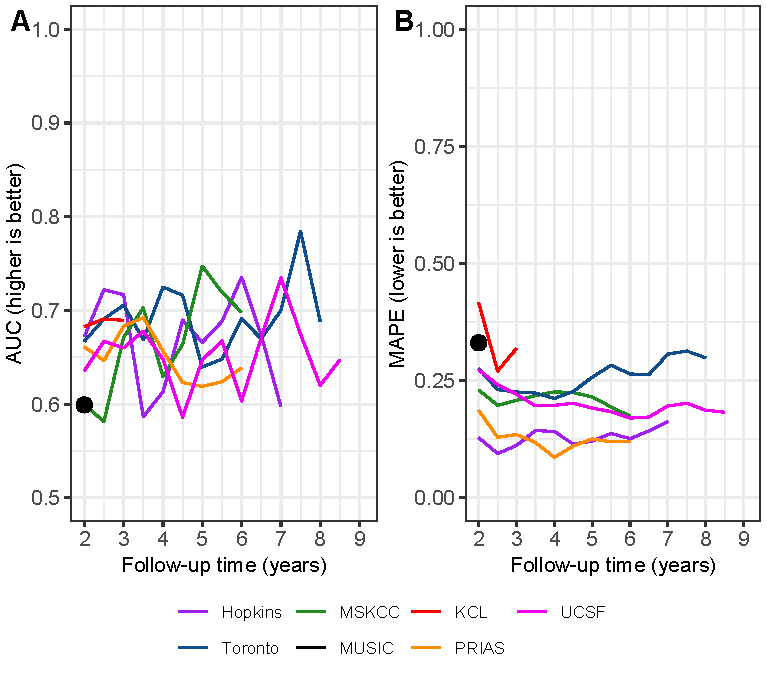
\includegraphics{contents/c5/images/c5_fig_app4.pdf}}
\caption{\textbf{Validation of dynamic predictions of cause-specific cumulative upgrading-risk}. In \textbf{Panel~A} area under the receiver operating characteristic curve or AUC (measure of discrimination) is between 0.6 and 0.7. \textbf{Panel~B} we can see that the time dependent root mean squared prediction error or MAPE is similar for PRIAS and Hopkins cohorts. The bootstrapped 95\% confidence interval for these estimates are presented in Table~\ref{c5:tab:AUC_PE_PRIAS} to Table~\ref{c5:tab:AUC_PE_KCL}. Full names of Cohorts are \textit{PRIAS}: Prostate Cancer International Active Surveillance, \textit{Toronto}: University of Toronto Active Surveillance, \textit{Hopkins}: Johns Hopkins Active Surveillance, \textit{MSKCC}: Memorial Sloan Kettering Cancer Center Active Surveillance, \textit{KCL}: King's College London Active Surveillance, \textit{MUSIC}: Michigan Urological Surgery Improvement Collaborative Active Surveillance, \textit{UCSF}: University of California San Francisco Active Surveillance.}
\label{c5:fig:auc_pe_recalib}
\end{figure}

\begin{table}
\small
\centering
\caption{\textbf{Internal validation of predictions of upgrading in PRIAS cohort}. The area under the receiver operating characteristic curve or AUC (measure of discrimination) and mean absolute prediction error or MAPE are calculated over the follow-up period at a gap of 6 months. In addition bootstrapped 95\% confidence intervals (CI) are also presented.}
\label{c5:tab:AUC_PE_PRIAS}
\begin{tabular}{r|r|r}
\hline
\hline
Follow-up period (years) & AUC (95\% CI) & MAPE (95\%CI)\\ 
\hline
1.0 to 2.0 & 0.661 [0.647, 0.678] & 0.187 [0.183, 0.191]\\
1.5 to 2.5 & 0.647 [0.596, 0.688] & 0.129 [0.122, 0.140]\\
2.0 to 3.0 & 0.683 [0.642, 0.723] & 0.135 [0.125, 0.146]\\
2.5 to 3.5 & 0.692 [0.632, 0.748] & 0.118 [0.111, 0.128]\\
3.0 to 4.0 & 0.657 [0.603, 0.709] & 0.086 [0.080, 0.092]\\
3.5 to 4.5 & 0.623 [0.582, 0.660] & 0.111 [0.105, 0.116]\\
4.0 to 5.0 & 0.619 [0.582, 0.654] & 0.126 [0.118, 0.131]\\
4.5 to 5.5 & 0.624 [0.537, 0.711] & 0.119 [0.103, 0.135]\\
5.0 to 6.0 & 0.639 [0.582, 0.696] & 0.121 [0.103, 0.138]\\
\hline
\end{tabular}    
\end{table}

\begin{table}
\small
\centering
\caption{\textbf{External validation of predictions of upgrading in University of Toronto Active Surveillance cohort}. The area under the receiver operating characteristic curve or AUC (measure of discrimination) and mean absolute prediction error or MAPE are calculated over the follow-up period at a gap of 6 months. In addition bootstrapped 95\% confidence intervals (CI) are also presented.}
\label{c5:tab:AUC_PE_Toronto}
\begin{tabular}{r|r|r}
\hline
\hline
Follow-up period (years) & AUC (95\% CI) & MAPE (95\%CI)\\ 
\hline
1.0 to 2.0 & 0.667 [0.634, 0.712] & 0.276 [0.259, 0.296]\\
1.5 to 2.5 & 0.691 [0.651, 0.730] & 0.231 [0.205, 0.254]\\
2.0 to 3.0 & 0.706 [0.637, 0.762] & 0.226 [0.196, 0.260]\\
2.5 to 3.5 & 0.669 [0.586, 0.741] & 0.224 [0.195, 0.258]\\
3.0 to 4.0 & 0.725 [0.649, 0.806] & 0.212 [0.184, 0.238]\\
3.5 to 4.5 & 0.716 [0.642, 0.793] & 0.227 [0.206, 0.258]\\
4.0 to 5.0 & 0.640 [0.579, 0.717] & 0.257 [0.222, 0.312]\\
4.5 to 5.5 & 0.648 [0.579, 0.740] & 0.283 [0.247, 0.326]\\
5.0 to 6.0 & 0.691 [0.608, 0.793] & 0.264 [0.232, 0.302]\\
5.5 to 6.5 & 0.670 [0.543, 0.776] & 0.263 [0.227, 0.307]\\
6.0 to 7.0 & 0.700 [0.544, 0.851] & 0.307 [0.258, 0.363]\\
6.5 to 7.5 & 0.785 [0.640, 0.866] & 0.313 [0.272, 0.360]\\
7.0 to 8.0 & 0.688 [0.532, 0.786] & 0.299 [0.249, 0.361]\\
\hline
\end{tabular}    
\end{table}

\begin{table}
\small
\centering
\caption{\textbf{External validation of predictions of upgrading in University of California San Francisco Active Surveillance cohort}. The area under the receiver operating characteristic curve or AUC (measure of discrimination) and mean absolute prediction error or MAPE are calculated over the follow-up period at a gap of 6 months. In addition bootstrapped 95\% confidence intervals (CI) are also presented.}
\label{c5:tab:AUC_PE_UCSF}
\begin{tabular}{r|r|r}
\hline
\hline
Follow-up period (years) & AUC (95\% CI) & MAPE (95\%CI)\\ 
\hline
1.0 to 2.0 & 0.635 [0.595, 0.677] & 0.273 [0.266, 0.281]\\
1.5 to 2.5 & 0.667 [0.628, 0.715] & 0.241 [0.224, 0.259]\\
2.0 to 3.0 & 0.660 [0.600, 0.713] & 0.221 [0.205, 0.238]\\
2.5 to 3.5 & 0.678 [0.614, 0.757] & 0.197 [0.175, 0.214]\\
3.0 to 4.0 & 0.648 [0.574, 0.707] & 0.197 [0.179, 0.221]\\
3.5 to 4.5 & 0.586 [0.525, 0.638] & 0.202 [0.180, 0.229]\\
4.0 to 5.0 & 0.647 [0.590, 0.754] & 0.192 [0.168, 0.217]\\
4.5 to 5.5 & 0.667 [0.582, 0.773] & 0.184 [0.159, 0.220]\\
5.0 to 6.0 & 0.603 [0.496, 0.696] & 0.170 [0.144, 0.207]\\
5.5 to 6.5 & 0.671 [0.576, 0.786] & 0.173 [0.145, 0.202]\\
6.0 to 7.0 & 0.735 [0.663, 0.794] & 0.196 [0.166, 0.219]\\
6.5 to 7.5 & 0.675 [0.565, 0.769] & 0.202 [0.168, 0.231]\\
7.0 to 8.0 & 0.620 [0.518, 0.740] & 0.187 [0.144, 0.217]\\
7.5 to 8.5 & 0.647 [0.538, 0.787] & 0.183 [0.146, 0.222]\\
\hline
\end{tabular}    
\end{table}

\begin{table}
\small
\centering
\caption{\textbf{External validation of predictions of upgrading in Johns Hopkins Active Surveillance cohort}. The area under the receiver operating characteristic curve or AUC (measure of discrimination) and mean absolute prediction error or MAPE are calculated over the follow-up period at a gap of 6 months. In addition bootstrapped 95\% confidence intervals (CI) are also presented.}
\label{c5:tab:AUC_PE_Hopkins}
\begin{tabular}{r|r|r}
\hline
\hline
Follow-up period (years) & AUC (95\% CI) & MAPE (95\%CI)\\ 
\hline
1.0 to 2.0 & 0.672 [0.604, 0.744] & 0.128 [0.115, 0.141]\\
1.5 to 2.5 & 0.722 [0.652, 0.792] & 0.095 [0.081, 0.111]\\
2.0 to 3.0 & 0.717 [0.638, 0.777] & 0.112 [0.100, 0.123]\\
2.5 to 3.5 & 0.587 [0.493, 0.704] & 0.144 [0.129, 0.154]\\
3.0 to 4.0 & 0.613 [0.486, 0.742] & 0.141 [0.126, 0.156]\\
3.5 to 4.5 & 0.690 [0.594, 0.783] & 0.115 [0.100, 0.133]\\
4.0 to 5.0 & 0.666 [0.572, 0.754] & 0.121 [0.104, 0.147]\\
4.5 to 5.5 & 0.688 [0.519, 0.779] & 0.137 [0.119, 0.161]\\
5.0 to 6.0 & 0.735 [0.676, 0.820] & 0.126 [0.102, 0.152]\\
5.5 to 6.5 & 0.674 [0.581, 0.765] & 0.143 [0.121, 0.172]\\
6.0 to 7.0 & 0.597 [0.472, 0.712] & 0.163 [0.126, 0.195]\\
\hline
\end{tabular}    
\end{table}

\begin{table}
\small
\centering
\caption{\textbf{External validation of predictions of upgrading in Memorial Sloan Kettering Cancer Center Active Surveillance cohort}. The area under the receiver operating characteristic curve or AUC (measure of discrimination) and mean absolute prediction error or MAPE are calculated over the follow-up period at a gap of 6 months. In addition bootstrapped 95\% confidence intervals (CI) are also presented.}
\label{c5:tab:AUC_PE_MSKCC}
\begin{tabular}{r|r|r}
\hline
\hline
Follow-up period (years) & AUC (95\% CI) & MAPE (95\%CI)\\ 
\hline
1.0 to 2.0 & 0.599 [0.518, 0.671]  & 0.230 [0.207, 0.256]\\
1.5 to 2.5 & 0.581 [0.504, 0.663]  & 0.198 [0.168, 0.235]\\
2.0 to 3.0 & 0.671 [0.599, 0.741]  & 0.208 [0.182, 0.232]\\
2.5 to 3.5 & 0.703 [0.610, 0.777]  & 0.218 [0.197, 0.246]\\
3.0 to 4.0 & 0.629 [0.499, 0.706]  & 0.226 [0.194, 0.259]\\
3.5 to 4.5 & 0.664 [0.589, 0.756]  & 0.225 [0.199, 0.262]\\
4.0 to 5.0 & 0.747 [0.642, 0.841]  & 0.215 [0.188, 0.247]\\
4.5 to 5.5 & 0.719 [0.597, 0.852]  & 0.194 [0.165, 0.232]\\
5.0 to 6.0 & 0.698 [0.565, 0.792]  & 0.174 [0.136, 0.227]\\
\hline
\end{tabular}    
\end{table}

\begin{table}
\small
\centering
\caption{\textbf{External validation of predictions of upgrading in King's College London Active Surveillance cohort}. The area under the receiver operating characteristic curve or AUC (measure of discrimination) and mean absolute prediction error or MAPE are calculated over the follow-up period at a gap of 6 months. In addition bootstrapped 95\% confidence intervals (CI) are also presented.}
\label{c5:tab:AUC_PE_KCL}
\begin{tabular}{r|r|r}
\hline
\hline
Follow-up period (years) & AUC (95\% CI) & MAPE (95\%CI)\\ 
\hline
1.0 to 2.0 & 0.683 [0.604, 0.753] & 0.416 [0.396, 0.445] \\
1.5 to 2.5 & 0.691 [0.621, 0.766] & 0.271 [0.246, 0.297] \\
2.0 to 3.0 & 0.689 [0.616, 0.785] & 0.319 [0.282, 0.344] \\
\hline
\end{tabular}    
\end{table}

\begin{table}
\small
\centering
\caption{\textbf{External validation of predictions of upgrading in Michigan Urological Surgery Improvement Collaborative Active Surveillance cohort}. The area under the receiver operating characteristic curve or AUC (measure of discrimination) and mean absolute prediction error or MAPE are calculated over the follow-up period at a gap of 6 months. In addition bootstrapped 95\% confidence intervals (CI) are also presented.}
\label{c5:tab:AUC_PE_MUSIC}
\begin{tabular}{r|r|r}
\hline
\hline
Follow-up period (years) & AUC (95\% CI) & MAPE (95\%CI)\\ 
\hline
1.0 to 2.0 & 0.599 [0.553, 0.632] & 0.331 [0.317, 0.348]\\
\hline
\end{tabular}    
\end{table}

\section{Source Code}
\label{c5:appendix:source_code}
The R code for fitting the joint model to the PRIAS dataset, is at \url{https://github.com/anirudhtomer/prias/tree/master/src/clinical_gap3}. We refer to this location as `R\_HOME' in the rest of this document. The PRIAS dataset is not openly accessible. However, access to the database can be requested via the contact links at \url{https://www.prias-project.org}.

The PRIAS dataset is in the so-called wide format and also requires the removal of incorrect entries. This can be done via the R script \url{R_HOME/dataset_cleaning.R}. This will lead to two R objects, namely `prias\_final.id' and `prias\_long\_final'. The `prias\_final.id' object contains information about the time of upgrading for PRIAS patients. The `prias\_long\_final' object contains longitudinal PSA measurements, the time of biopsies and results of biopsies.

We use a joint model for time-to-event and longitudinal data to model the evolution of PSA measurements over time, and to simultaneously model their association with the risk of upgrading. The R package we use for this purpose is called \textbf{JMbayes} (https://cran.r-project.org/web/packages/JMbayes/JMbayes.pdf). The API we use, however, is currently not hosted on CRAN, and can be found here:
\url{https://github.com/anirudhtomer/JMbayes}. The joint model can be fitted via the script \url{R_HOME/analysis.R}. It takes roughly 6 hours to run on an Intel Core-i5 machine with four cores and 8GB of RAM. 

The graphs presented in the main manuscript, and the appendix can be generated by the scripts in \url{R_HOME/plots/}.

Validations can be done using the scripts \url{R_HOME/validation/auc_brier/auc_calculator.R}, and \url{R_HOME/validation/auc_brier/gof_calculator.R}. For external validation access to GAP3 database is required.

Once a joint model is fitted to the PRIAS dataset, personalized schedules of biopsies based on the risk of upgrading for new patients can be developed as shown in the script \url{R_HOME/plots/demo_schedule_supplementary.R} or directly using the script \url{https://raw.githubusercontent.com/anirudhtomer/prias/master/src/lastpaper/pers_schedule_api.R}.

Source code for the shiny web application which provides biopsy schedules for patients can be found at \url{R_HOME/shinyapp}
\end{subappendices}